% https://es.overleaf.com/latex/templates/project-report/jpzczmpsdzwm

%%% Preamble
\documentclass[paper=leter, fontsize=11pt]{scrartcl}
\usepackage[utf8]{inputenc}
\usepackage[spanish,mexico]{babel}
\usepackage[T1]{fontenc}    % use 8-bit T1 fonts
\usepackage{lmodern}
\usepackage{hyperref}       % hyperlinks
\usepackage{lipsum}
\usepackage[square,numbers]{natbib}
\usepackage{enumitem}

\usepackage[protrusion=true,expansion=true]{microtype}	
\usepackage{amsmath,amsfonts,amsthm} % Math packages
\usepackage[pdftex]{graphicx}
\usepackage{url}
% https://tex.stackexchange.com/a/3785
\usepackage{breqn}
 
\usepackage{booktabs}
\usepackage[table,xcdraw]{xcolor}

\usepackage{tikz}
\usetikzlibrary{positioning,matrix, arrows.meta}

\usepackage{caption} 
\usepackage{subcaption}

\usepackage{multirow}

\usepackage{listings}
\lstdefinestyle{mystyle}{ 
    language=R,
    basicstyle=\ttfamily\footnotesize,
    breakatwhitespace=false,         
    breaklines=true,                 
    captionpos=b,                    
    keepspaces=true,                 
    numbers=left,                    
    numbersep=5pt,                  
    showspaces=false,                
    showstringspaces=false,
    showtabs=false,                  
    tabsize=2
}

\lstset{style=mystyle}
\renewcommand{\lstlistingname}{Código}


\selectlanguage{spanish}
\usepackage[spanish,onelanguage,ruled]{algorithm2e}


%%% Custom sectioning
\usepackage{sectsty}
\allsectionsfont{\centering \normalfont\scshape}


%%% Custom headers/footers (fancyhdr package)
\usepackage{fancyhdr}
\pagestyle{fancyplain}
\fancyhead{}											% No page header
\fancyfoot[L]{}											% Empty 
\fancyfoot[C]{}											% Empty
\fancyfoot[R]{\thepage}									% Pagenumbering
\renewcommand{\headrulewidth}{0pt}			% Remove header underlines
\renewcommand{\footrulewidth}{0pt}				% Remove footer underlines
\setlength{\headheight}{13.6pt}


%%% Equation and float numbering
%\numberwithin{equation}{section}		    % Equationnumbering: section.eq#
%\numberwithin{figure}{section}			    % Figurenumbering: section.fig#
%\numberwithin{table}{section}				% Tablenumbering: section.tab#

%\newtheorem{thm}{Theorem}
%\newtheorem{prop}{Proposition}
%\newtheorem{lemma}{Lemma}
\newtheorem{ex}{Exercise}

%%% Maketitle metadata
\newcommand{\horrule}[1]{\rule{\linewidth}{#1}} 	% Horizontal rule

%%% https://tex.stackexchange.com/a/118217
\usepackage{mathtools}
\DeclarePairedDelimiter\ceil{\lceil}{\rceil}
\DeclarePairedDelimiter\floor{\lfloor}{\rfloor}

\title{
		%\vspace{-1in} 	
		\usefont{OT1}{bch}{b}{n}
		\normalfont \normalsize \textsc{Posgrado de Ingeniería de Sistemas} \\ [25pt]
		\horrule{0.5pt} \\[0.4cm]
		\huge Teorema del límite central \\
		\horrule{2pt} \\[0.5cm]
}
\author{
		\normalfont 								\normalsize
        Alberto Benavides\\[-3pt]		\normalsize
        \today
}
\date{}


%%% Begin document
\begin{document} 
\maketitle

\section{Introducción}

El \textbf{teorema del límite central} expresa que conforme la media $\bar{X_n}$ de $n$ variables aleatorias independientes e idénticamente distribuidas $X_i$ de una distribución $D$ cualquiera, se aproxima a una distribución normal con media $\mu$ y varianza $\sigma^2$ relacionados con la distribución $D$ conforme $n$ tiende a $+\infty$. Esto se puede mostrar experimentalmente partiendo, por ejemplo, de una distribución exponencial generada a partir de la función \texttt{rexp} del lenguaje de programación R. El histograma de mil valores obtenidos al azar de dicha distribución aparece en la figura \ref{fig:rexp} (p. \pageref{fig:rexp}). De dicha distribución se pueden obtener muestras de distintos tamaños, en este caso $n = [2, 10, 30, 50]$, con lo que mostrar cómo estas distribuciones se aproximan a una distribución normal. Para este fin, se plasman los histogramas para cada $n$ en la figura \ref{fig:ejemplos} (p. \pageref{fig:ejemplos}).

\begin{figure}
  \centering
  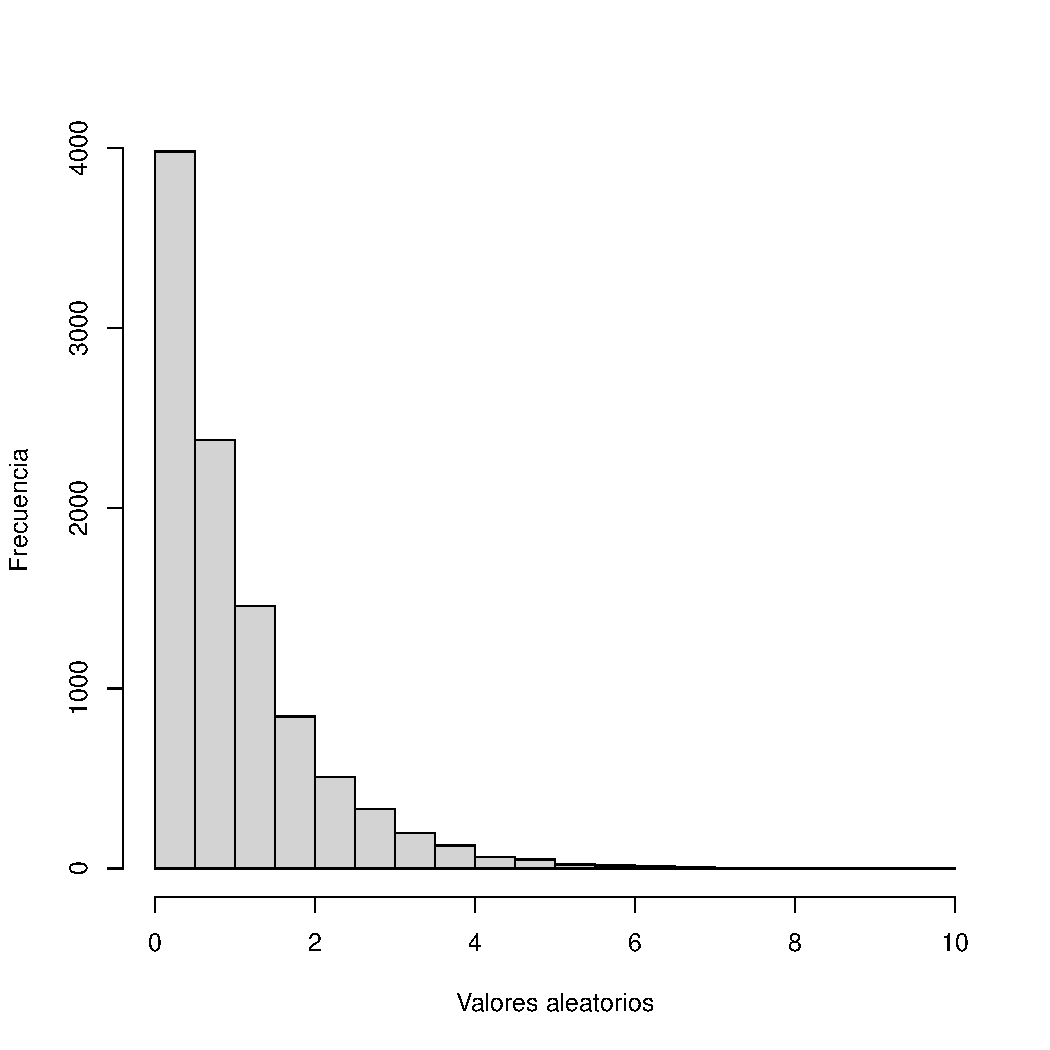
\includegraphics[width=0.8\textwidth]{rexp.pdf}
\caption{Histograma de mil valores obtenidos de una distribución exponencial con $\lambda = 1$.}
\label{fig:rexp}
\end{figure}

\begin{figure}
  \begin{subfigure}{.5\textwidth}
      \centering
      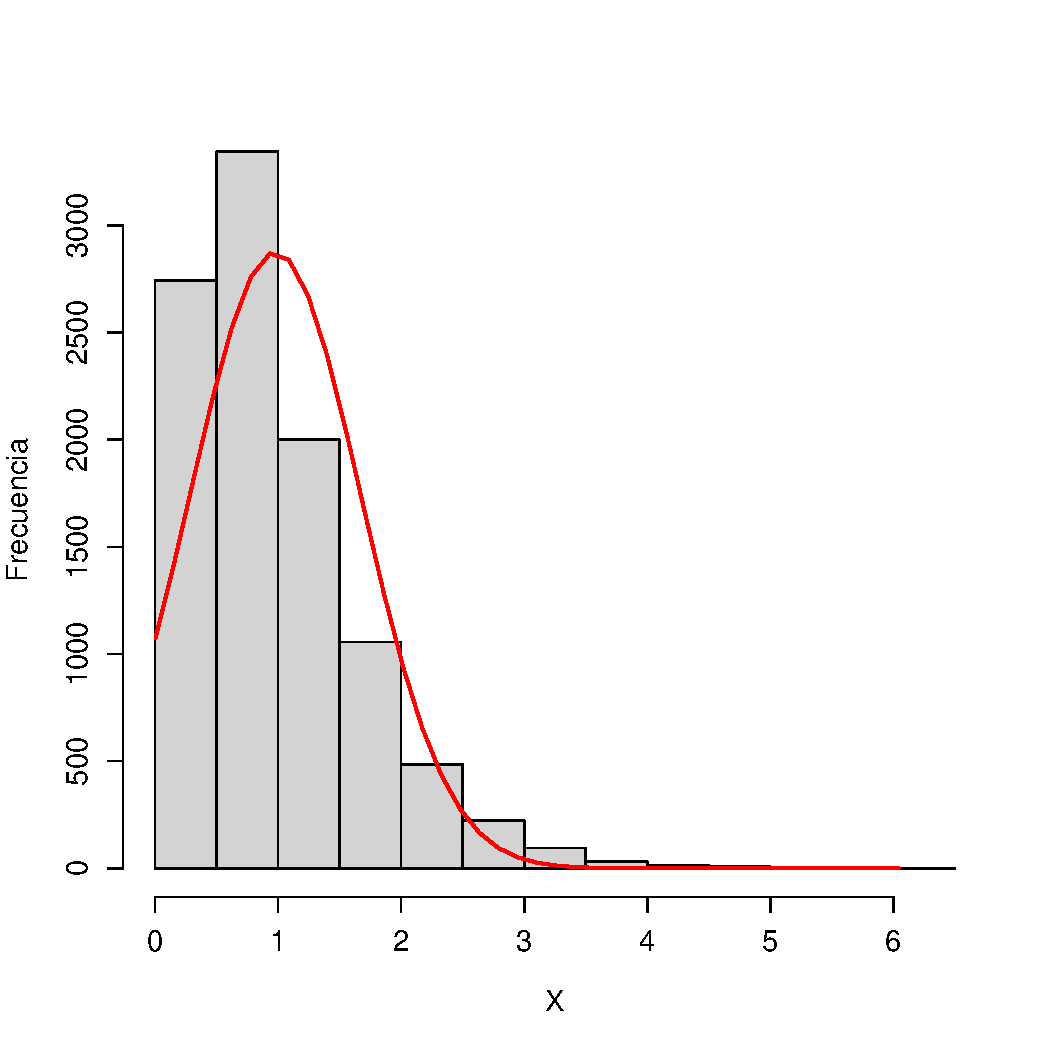
\includegraphics[scale=0.4]{ej_2.pdf}
      \caption{$n = 2$.}
  \end{subfigure}
  \begin{subfigure}{.5\textwidth}
      \centering
      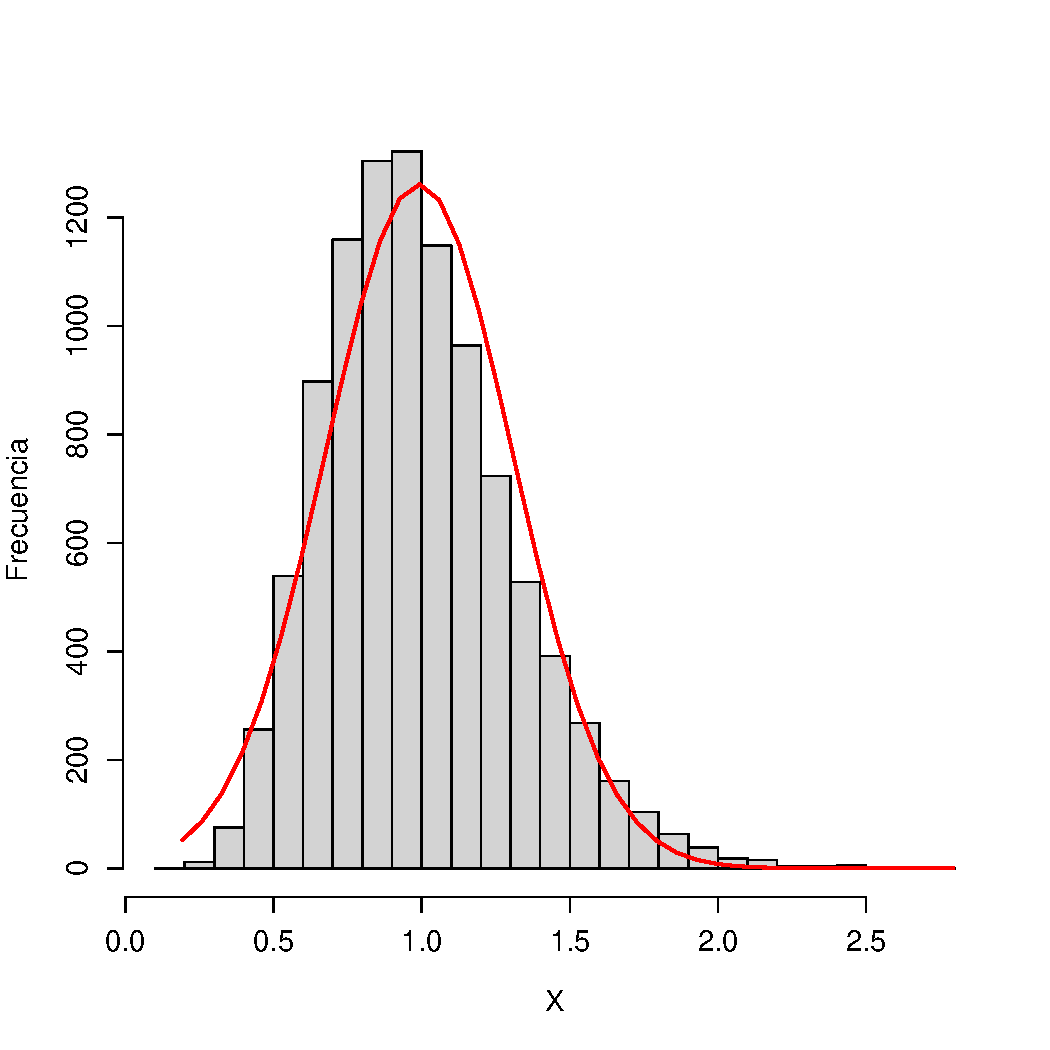
\includegraphics[scale=0.4]{ej_10.pdf}
      \caption{$n = 10$.}
  \end{subfigure}
  \begin{subfigure}{.5\textwidth}
    \centering
    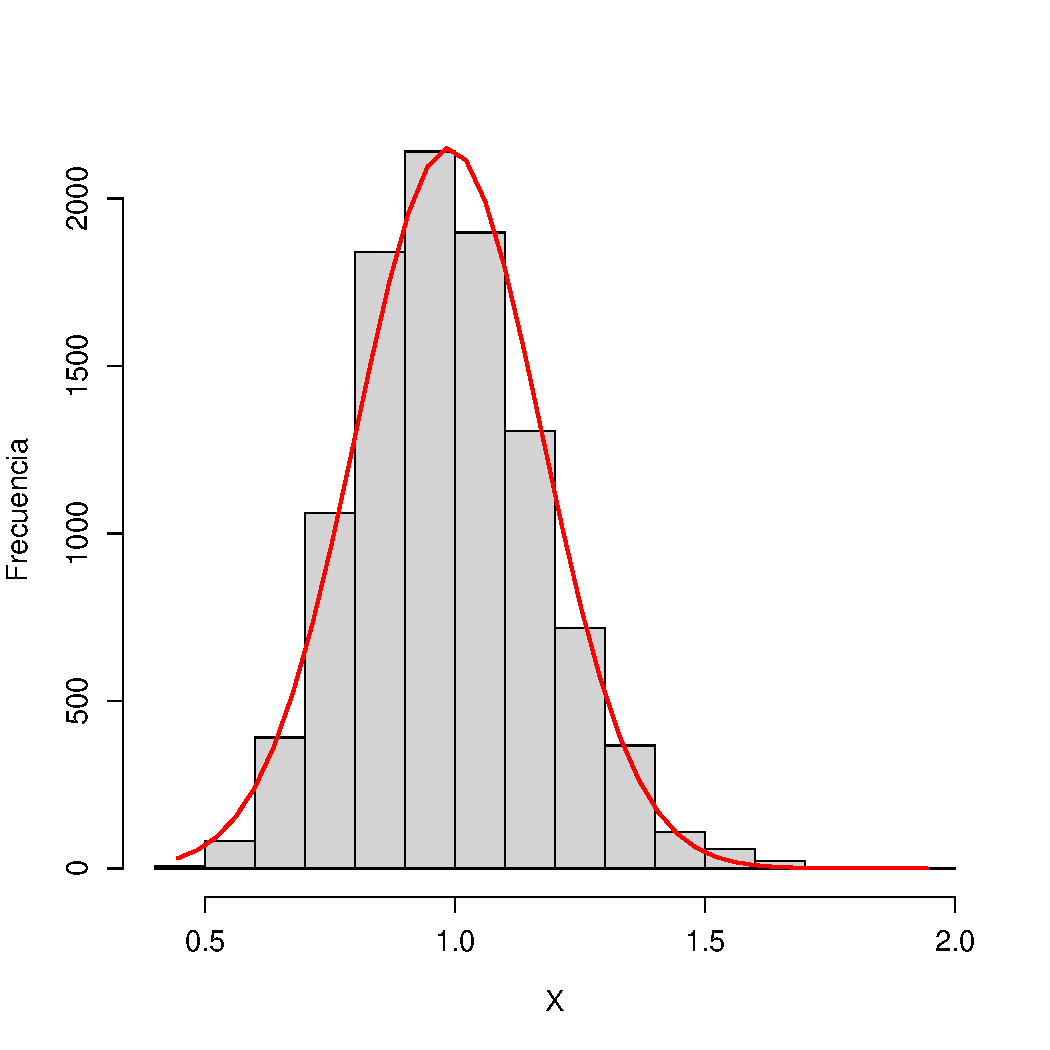
\includegraphics[scale=0.4]{ej_30.pdf}
    \caption{$n = 30$.}
\end{subfigure}
\begin{subfigure}{.5\textwidth}
  \centering
  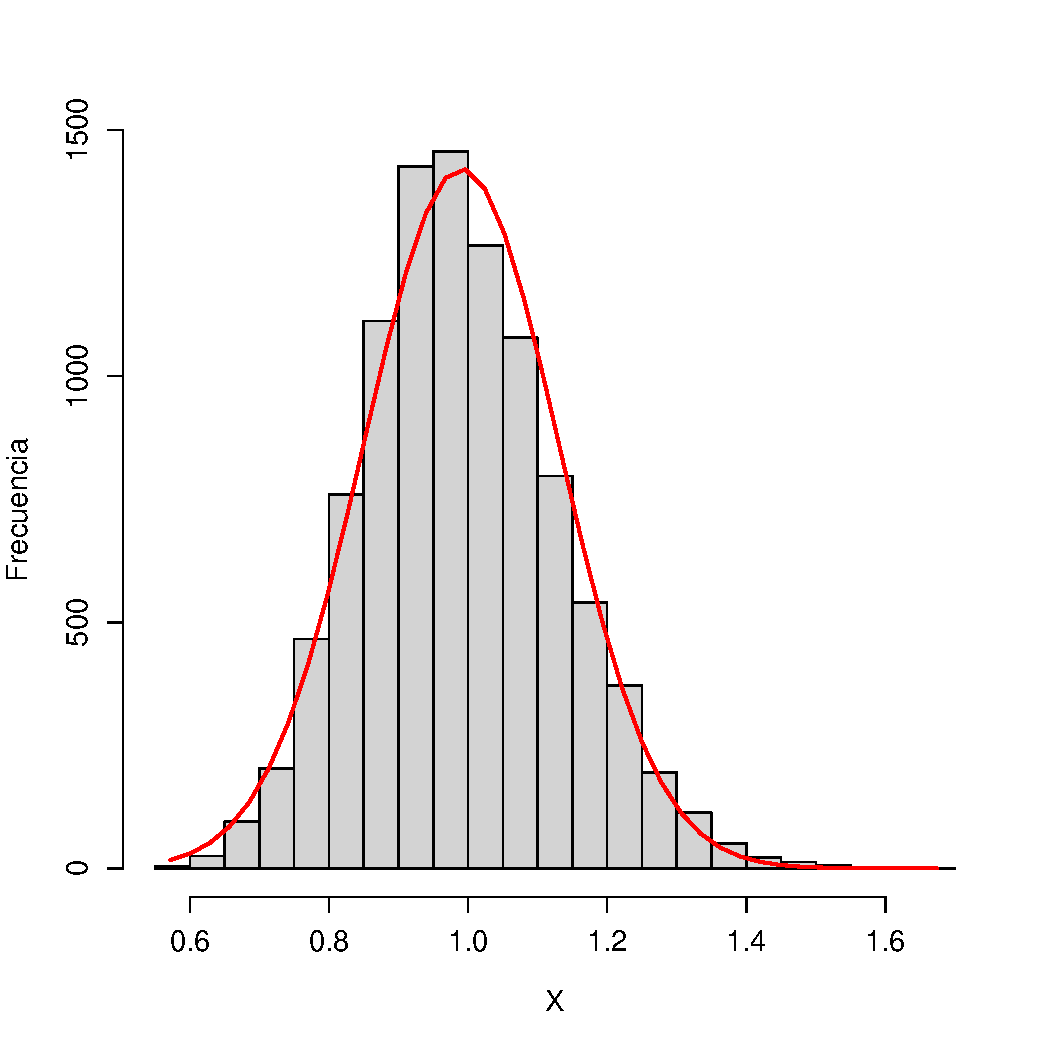
\includegraphics[scale=0.4]{ej_50.pdf}
  \caption{$n = 50$.}
\end{subfigure}
  \caption{Distribuciones de muestras con $n = [2, 10, 30, 50]$ variables aleatorias, con densidad teórica (línea roja) superpuesta.}
  \label{fig:ejemplos}
\end{figure}

\section{Aplicación}

Actualmente en México existe una normativa que se utiliza para comunicar la calidad del aire, publicada por la \citet{semarnat}. De entre los contaminantes que regula, se encuentra el material particulado con tamaño menor o igual a $10\ \mu\text{g}$, contaminante denominado como PM10. Este tipo de partículas están asociadas con riesgos pulmonares, cardiovasculares e incluso con muertes prematuras. El \citet{aireNL} registra cada segundo, mediante trece estaciones de monitoreo meteorológico, la concentración de PM10 medida en $\mu\text{g} / \text{m}^3$. La norma establece que a partir de $50\ \mu\text{g} / \text{m}^3$ de concentración de PM10 promediadas por cada doce horas es que aparecen síntomas y afecciones que son clasificados como \emph{malas}. En la figura \ref{fig:pm10} (p. \pageref{fig:pm10}) aparecen la serie de tiempo\footnote{\url{https://es.wikipedia.org/wiki/Serie_temporal}} y el histograma de estas concentraciones, acompañadas por una recta roja que indica el nivel a partir del cual se consideran \emph{mala} la cantidad de contaminantes. 

\begin{figure}
  \begin{subfigure}{.8\textwidth}
    \centering
    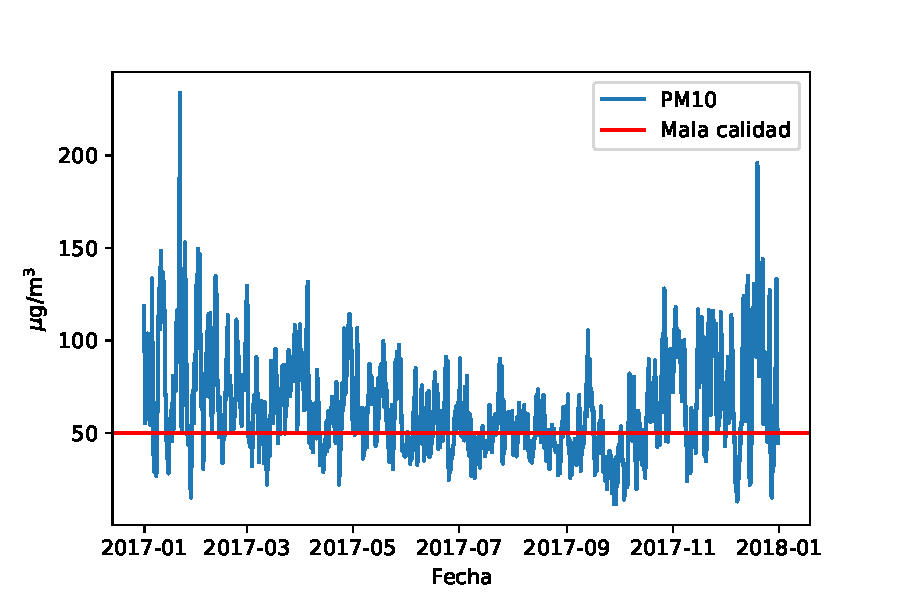
\includegraphics{ts_2017_pm10.pdf}
    \caption{Serie de tiempo.}
\end{subfigure}
  \begin{subfigure}{.8\textwidth}
      \centering
      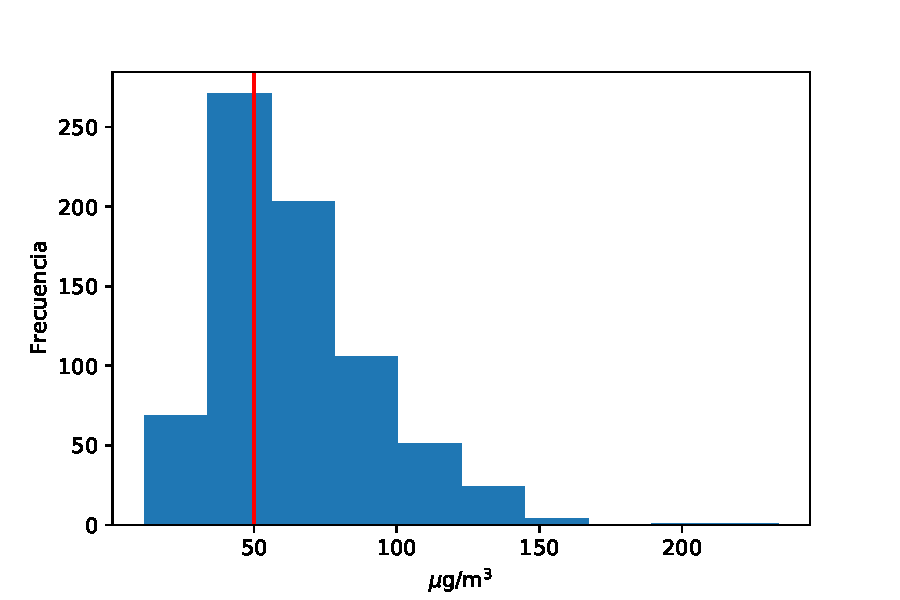
\includegraphics{hist_2017_pm10.pdf}
      \caption{Histograma.}
  \end{subfigure}
  \caption{Serie de tiempo e histograma de las concentraciones en promedio por cada doce horas de PM10 durante 2017 en el área metropolitana de Monterrey.}
  \label{fig:pm10}
\end{figure}

Una justificación de un estudio sobre estos contaminantes podría obtenerse mediante el teorema del límite central. Así, se puede preguntar cuál es la probabilidad de que de una muestra suficientemente grande de las concentraciones de esos valores esté por encima de lo considerado como \emph{malo}, o sea $50 \mu\text{g} / \text{m}^3$. A partir del teorema del límite central, se puede considerar que dicha muestra tendrá una distribución normal con $\mu = 64.03$ y $\sigma^2 = 27.82$ calculadas a partir de los registros. Finalmente, mediante \texttt{pnorm(50, 64.03, 27.82, lower.tail = F)} se calcula $P\left(\frac{\bar{X} - 64.03}{27.82} \geq 50\right) = 0.69$, es decir que teóricamente se puede esperar con un $69\%$ de probabilidades, encontrar concentraciones \emph{malas} al tomar muestras de manera aleatoria entre los registros de PM10 durante 2017 en el Área Metropolitana de Monterrey, lo que motiva su análisis y exploración de la relación entre estos contaminantes y las afecciones que pudieran ocasionar.

\bibliographystyle{mighelnat}
\bibliography{Biblio}

\end{document}